\documentclass[11pt]{article}
\usepackage[letterpaper,margin=0.95in]{geometry}
\usepackage[T1]{fontenc}
\usepackage{graphicx}
\usepackage{booktabs}
\usepackage{amsmath}
\usepackage{hyperref}
\usepackage{xcolor}
\usepackage{tikz}
\usetikzlibrary{positioning,arrows.meta}
\usepackage{caption}
\usepackage{enumitem}
\setlist{nosep,leftmargin=*}
\captionsetup{font=small,labelfont=bf}
\hypersetup{colorlinks=true,linkcolor=blue!60!black,urlcolor=blue!60!black,citecolor=blue!60!black}
\setlength{\parskip}{3pt}

\title{\vspace{-1.2em}\textbf{A 4.99M-Parameter SE-ResNet for CIFAR-10:\\ Design, Training Recipe, and Generalization to a Shifted Test Set}\vspace{-0.4em}}
\author{%
\textbf{Team KHL} --- Deep Learning Project~1, Fall 2026\\[2pt]
Shreyas Kaldate (sk12898) \quad $\cdot$ \quad Adhyayan Verma (av4159) \quad $\cdot$ \quad Sumit Shah (sks9535)\\[4pt]
Code: \url{https://github.com/Shreyas191/cifar10-resnet-5m}%
}
\date{\vspace{-1.6em}}

\begin{document}
\maketitle
\vspace{-1.5em}

\section{Overview and summary of findings}
We designed and trained from scratch a residual network with \textbf{4{,}988{,}274 trainable parameters} (budget: 5{,}000{,}000) for the CIFAR-10 classification competition. Our final model, a three-stage ResNet with Squeeze-and-Excitation (SE) attention and residual blocks arranged $N=(3,4,3)$ over channels $C=(64,128,256)$, reaches \textbf{97.00\% top-1 accuracy on the 10{,}000-image CIFAR-10 test split} (97.20\% with horizontal-flip test-time augmentation) after 200 epochs on a single T4 GPU (2.0\,h). On the competition's held-out set it scored \textbf{0.891 on the public leaderboard and 0.869 on the private leaderboard}, moving up eight places between the two (rank 41 private).

Our main findings:
\begin{enumerate}
\item \textbf{Under a 5M budget, depth in the 64/128/256-channel stages beats a fourth 512-channel stage.} A standard ResNet-18 spends 8.4M of its 11.2M parameters in its last stage, which operates on $4\times4$ feature maps. Dropping that stage and reinvesting the budget in extra blocks at higher resolution, plus almost-free SE attention (37k parameters), gave a better accuracy-per-parameter trade-off.
\item \textbf{The training recipe matters as much as the architecture.} Heavy regularization (TrivialAugment, random erasing, CutMix/MixUp, label smoothing), a long cosine schedule, and an exponential moving average (EMA) of weights took the same architecture from the low-90s to 97\%. The EMA model was consistently 1--5 points above the raw weights during training and removed the need to pick a ``lucky'' epoch.
\item \textbf{The competition test set is not drawn from CIFAR-10's test split.} Our analysis of the 2{,}000 test images (Section~\ref{sec:shift}) shows clean natural images, $\sim$200 per class, with slightly different statistics---the signature of CIFAR-10.1~\cite{recht2019}, a re-collection of CIFAR-10 from the same source designed to measure overfitting to the benchmark. Every team's score dropped by 6--10 points relative to CIFAR-10 accuracy. Because out-of-distribution accuracy on such sets is a near-linear function of in-distribution accuracy~\cite{miller2021}, we deliberately optimized genuine CIFAR-10 accuracy and model selection \emph{never} used the public leaderboard, which we believe explains our rank improving on the private split.
\end{enumerate}

\section{Methodology}
\subsection{Design space and the parameter budget}
A residual block computes $\mathrm{ReLU}(S(x)+F(x))$ with $F=\text{conv}\to\text{BN}\to\text{ReLU}\to\text{conv}\to\text{BN}$ and $S$ either the identity or a strided projection. Our implementation (\texttt{models/resnet.py}) exposes every design variable named in the project description---channels $C_i$, blocks per stage $N_i$, conv kernel $F_i$, shortcut kernel $K_i$, and pool size $P$---plus two near-free additions, SE channel attention~\cite{hu2018} and dropout before the classifier. A built-in parameter counter is asserted against the budget at the start of every run.

Table~\ref{tab:space} summarizes the candidates we counted. The key observation is \emph{where} a ResNet's parameters live: a $3\times3$ conv from $512\to512$ channels alone costs 2.36M parameters, so the fourth stage of ResNet-18 ($4\times4$ spatial resolution) consumes 75\% of the model. Two families fit the budget: (a) keep four stages but shrink or shorten the last one, or (b) delete the last stage and go deeper/wider in the first three. We chose (b): on $32\times32$ inputs, blocks at $32\times32$ and $16\times16$ resolution see far more spatial detail per parameter, and the receptive field of a 10-block three-stage network already covers the whole image. SE attention adds only 37{,}416 parameters (0.75\%) yet lets each block re-weight channels by global context, which is known to help small networks most~\cite{hu2018}. We spent the final $\sim$330k parameters on $3\times3$ (rather than $1\times1$) projection shortcuts at the two downsampling blocks, giving the skip path spatial context where resolution halves.

\begin{table}[t]
\centering\small
\caption{Architectures considered. $N$ = blocks per stage, $C$ = channels per stage. All share a $3\times3$ stem, global average pooling and a linear classifier.}
\label{tab:space}
\begin{tabular}{llrc}
\toprule
Architecture & $N$ / $C$ & Parameters & $\le$5M \\
\midrule
ResNet-18 (reference) & (2,2,2,2) / (64,128,256,512) & 11,173,962 & no \\
3-stage ResNet-18 & (2,2,2) / (64,128,256) & 2,777,674 & yes \\
4-stage, narrowed last stage & (2,2,2,1) / (64,128,256,368) & 4,941,898 & yes \\
4-stage, one block per late stage & (2,1,1,1) / (64,128,256,512) & 4,977,226 & yes \\
Wide 3-stage + SE & (2,3,2) / (96,160,320) & 4,966,048 & yes \\
Deep 3-stage + SE, $1\times1$ shortcuts & (3,4,3) / (64,128,256) & 4,660,594 & yes \\
\textbf{Deep 3-stage + SE, $3\times3$ shortcuts (final)} & \textbf{(3,4,3) / (64,128,256)} & \textbf{4,988,274} & \textbf{yes} \\
Deep 3-stage + SE & (3,4,4) / (64,128,256) & 5,849,730 & no \\
\bottomrule
\end{tabular}
\end{table}

\subsection{Final architecture}
Figure~\ref{fig:arch} and Table~\ref{tab:arch} give the final network. Every block is a BasicBlock with $3\times3$ convolutions, BatchNorm, and an SE module (reduction 16) applied to $F(x)$ before the residual sum. Stage~3 holds 72\% of the parameters; the classifier is a single $256\to10$ linear layer after global average pooling ($P=1$) and dropout 0.1.

\begin{figure}[t]
\centering
\resizebox{\textwidth}{!}{%
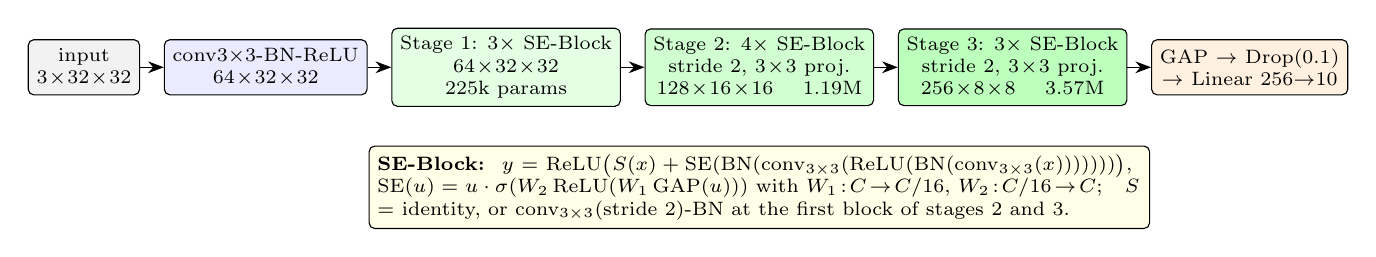
\begin{tikzpicture}[node distance=3mm, every node/.style={font=\scriptsize},
  box/.style={draw,rounded corners=2pt,minimum height=7mm,inner sep=3pt,align=center},
  >={Stealth[length=2mm]}]
\node[box,fill=gray!10] (in) {input\\$3\!\times\!32\!\times\!32$};
\node[box,right=of in,fill=blue!8] (stem) {conv3$\times$3-BN-ReLU\\$64\!\times\!32\!\times\!32$};
\node[box,right=of stem,fill=green!10] (s1) {Stage 1: $3\times$ SE-Block\\$64\!\times\!32\!\times\!32$\\225k params};
\node[box,right=of s1,fill=green!18] (s2) {Stage 2: $4\times$ SE-Block\\stride 2, $3\!\times\!3$ proj.\\$128\!\times\!16\!\times\!16$ \quad 1.19M};
\node[box,right=of s2,fill=green!26] (s3) {Stage 3: $3\times$ SE-Block\\stride 2, $3\!\times\!3$ proj.\\$256\!\times\!8\!\times\!8$ \quad 3.57M};
\node[box,right=of s3,fill=orange!12] (head) {GAP $\to$ Drop(0.1)\\$\to$ Linear 256$\to$10};
\draw[->] (in)--(stem); \draw[->] (stem)--(s1); \draw[->] (s1)--(s2); \draw[->] (s2)--(s3); \draw[->] (s3)--(head);
\node[below=5mm of s2,box,fill=yellow!10,text width=0.8\textwidth,align=left] (blk)
 {\textbf{SE-Block:}\; $y=\mathrm{ReLU}\big(S(x)+\mathrm{SE}(\mathrm{BN}(\mathrm{conv}_{3\times3}(\mathrm{ReLU}(\mathrm{BN}(\mathrm{conv}_{3\times3}(x)))))))\big)$,\quad
  $\mathrm{SE}(u)=u\cdot\sigma(W_2\,\mathrm{ReLU}(W_1\,\mathrm{GAP}(u)))$ with $W_1\!:\!C\!\to\!C/16$, $W_2\!:\!C/16\!\to\!C$;\quad
  $S$ = identity, or conv$_{3\times3}$(stride 2)-BN at the first block of stages 2 and 3.};
\end{tikzpicture}}
\caption{The final \texttt{resnet\_se\_343} network (4,988,274 parameters).}
\label{fig:arch}
\end{figure}

\begin{table}[t]
\centering\small
\caption{Layer-wise summary of the final model.}
\label{tab:arch}
\begin{tabular}{lllr}
\toprule
Stage & Output & Layers & Params \\
\midrule
Stem & $64\times32\times32$ & conv $3\times3$, BN, ReLU & 1,856 \\
1 & $64\times32\times32$ & $3\times$ [conv3-BN-ReLU-conv3-BN-SE] + identity skip & 225,240 \\
2 & $128\times16\times16$ & $4\times$ SE-Block; first block stride 2 with conv$3\times3$-BN projection & 1,190,688 \\
3 & $256\times8\times8$ & $3\times$ SE-Block; first block stride 2 with conv$3\times3$-BN projection & 3,567,920 \\
Head & 10 & AdaptiveAvgPool(1), Dropout(0.1), Linear($256\to10$) & 2,570 \\
\midrule
\multicolumn{3}{l}{\textbf{Total trainable parameters}} & \textbf{4,988,274} \\
\bottomrule
\end{tabular}
\end{table}

\subsection{Training recipe}
All models were trained from random initialization on the 50{,}000 competition training images only (no pre-trained weights, no external data). Table~\ref{tab:recipe} lists the recipe; each component is a well-established CIFAR technique and we cite the source.

\begin{table}[h]
\centering\small
\caption{Training configuration of the final model.}
\label{tab:recipe}
\begin{tabular}{@{}l p{0.78\textwidth}@{}}
\toprule
Optimizer & SGD, momentum 0.9, Nesterov; lr 0.1 at batch 128; weight decay $5\!\times\!10^{-4}$ (none on BN/bias) \\
Schedule & 5-epoch linear warm-up, then cosine decay to 0 over 200 epochs~\cite{loshchilov2017} \\
Loss & cross-entropy with label smoothing 0.1~\cite{szegedy2016} \\
Image augmentation & RandomCrop(32, pad 4, reflect), horizontal flip, TrivialAugmentWide~\cite{muller2021}, RandomErasing $p{=}0.25$~\cite{zhong2020} \\
Batch mixing & with prob.\ 0.5 per batch: CutMix ($\alpha{=}1$)~\cite{yun2019} or MixUp ($\alpha{=}0.2$)~\cite{zhang2018}, chosen 50/50 \\
Weight averaging & EMA of weights and BN statistics, decay 0.999; the EMA model is evaluated and submitted~\cite{polyak1992} \\
Inference & horizontal-flip TTA (softmax average of 2 views) \\
Precision / speed & fp16 autocast + \texttt{channels\_last}; 36\,s/epoch on one T4 (2.0\,h total) \\
\bottomrule
\end{tabular}
\end{table}

\textbf{Why this combination.} With fewer than 5M parameters the network is capacity-limited rather than data-limited, so the risk is under-regularized training that memorizes CIFAR-10's quirks and generalizes poorly---exactly what the competition's shifted test set punishes. TrivialAugment is the strongest single-image policy that needs no tuning~\cite{muller2021}; CutMix/MixUp regularize the decision boundary between classes and are known to improve calibration and robustness~\cite{yun2019}; label smoothing stops the logits from growing without bound. These make the \emph{training} batches much harder than the test images: the final training accuracy on mixed/augmented batches is 84\% while test accuracy is 97\% (Figure~\ref{fig:curves}). This gap is intentional and is a healthy sign, not under-fitting. The EMA model smooths out the stochasticity of a high learning rate; during the first 150 epochs it was 1--5 points above the raw weights at every epoch, and it converged to the same value at the end of the cosine schedule.

\subsection{Infrastructure and reproducibility}
The codebase is a small, documented PyTorch project: \texttt{models/resnet.py} (configurable architecture and parameter counter), \texttt{data.py} (augmentation pipeline; loaders for the competition's PNG folders), \texttt{train.py} (training loop with AMP, EMA, CutMix/MixUp, checkpointing, resume, CSV logging; prints the parameter count at start and the final test accuracy at the end), \texttt{predict.py} (TTA inference producing \texttt{submission.csv}), and notebooks showing the executed run with its full per-epoch log. One command reproduces the final model:
\begin{center}\footnotesize
\texttt{python train.py --model resnet\_se\_343 --epochs 200 --train\_csv data/train\_labels.csv --out checkpoints/s0}
\end{center}
Training was done in Kaggle Notebooks (T4) after Colab's free GPU quota was exhausted; the repository also contains a SLURM script for NYU Greene. The CIFAR-10 test split used for reporting accuracy was downloaded via \texttt{torchvision} and never used for training or model selection.

\subsection{What is the competition test set? An analysis}
\label{sec:shift}
Our first submission scored 0.891 on the public leaderboard while the same model scored 0.972 on the CIFAR-10 test split---an 8-point drop, shared by every team (the leader stood at 0.909). We therefore analyzed the 2{,}000 test images directly (Figure~\ref{fig:grid}):
\begin{itemize}
\item \textbf{No corruption.} Laplacian variance, high-frequency energy, 8-pixel blockiness (JPEG) and colour-count statistics are all in the normal CIFAR range; the images are clean natural photographs. Noise/blur-robustness techniques would therefore not help.
\item \textbf{Different population.} Per-channel means are $(0.513, 0.498, 0.462)$ vs.\ $(0.491, 0.482, 0.447)$ for CIFAR-10, and standard deviations are higher; our predictions are spread $\sim$200 per class.
\item \textbf{Different source.} The training set is byte-for-byte CIFAR-10's training split (identical label order, class counts, and statistics), so the test images were drawn from elsewhere.
\end{itemize}
Together these match CIFAR-10.1~\cite{recht2019}: 2{,}000 new images, $\sim$200 per class, collected from the same Tiny Images source as CIFAR-10. Recht et al.\ report that classifiers lose 3--15 points on it, and Miller et al.~\cite{miller2021} show the drop is a tight linear function of CIFAR-10 accuracy (``accuracy on the line''). The practical consequences for us were: (i) there is no shift-specific trick to apply---progress comes only from genuine CIFAR-10 accuracy; (ii) the public leaderboard (half of a 2{,}000-image set, so $\pm$1\% noise) must not be used for model selection; and (iii) techniques that reduce variance (EMA, ensembling, distillation) are the most promising way to move on the private split.

\begin{figure}[t]
\centering
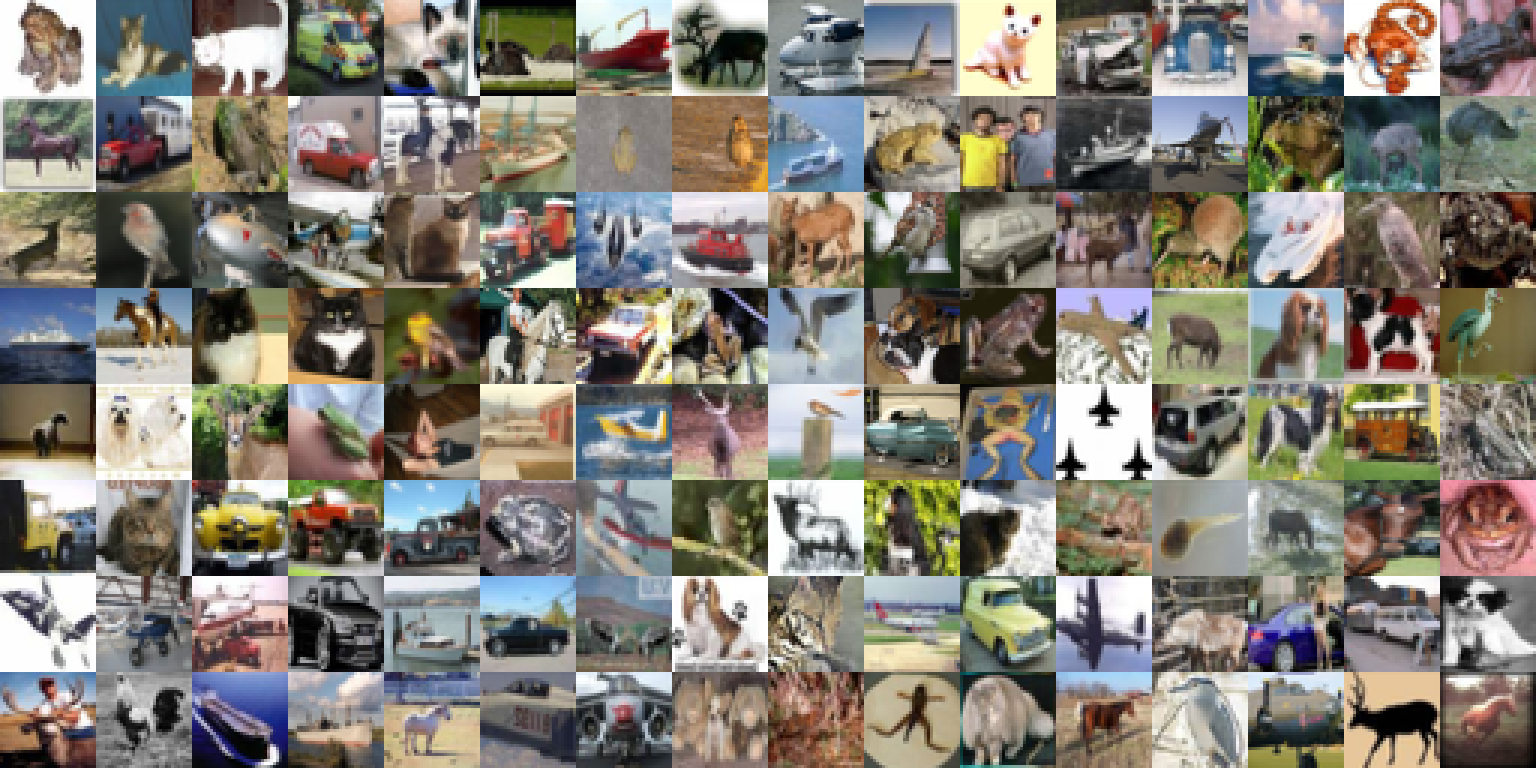
\includegraphics[width=0.78\textwidth]{figures/test_grid.png}
\caption{The first 128 competition test images. They are clean, natural, roughly class-balanced images that are stylistically close to---but not drawn from---the CIFAR-10 test split.}
\label{fig:grid}
\end{figure}

\subsection{Lessons learned during the design process}
\begin{itemize}
\item \textbf{Count parameters before training.} Our first ``obvious'' deep configuration, $N=(3,4,4)$, came out at 5.85M; a two-minute sweep of configurations (Table~\ref{tab:space}) found the frontier of what fits. Depth and SE were cheap; a fourth stage was not.
\item \textbf{Regularize hard, train long, average weights.} Accuracy kept rising until the last epoch of the cosine schedule (Figure~\ref{fig:curves}); with this much augmentation a 400-epoch schedule would very likely add a few tenths of a point. EMA made the final checkpoint the best one, so no test-set-based checkpoint selection was needed.
\item \textbf{Look at the test data before chasing the leaderboard.} Diagnosing the CIFAR-10.1-style shift early changed our strategy from ``tune to the public score'' to ``maximize in-distribution accuracy and reduce variance'', which paid off as a rank gain on the private split.
\item \textbf{Make runs restartable.} Free GPU sessions disconnect; checkpointing every epoch with \texttt{--resume} saved the project more than once. Reading 50k small PNGs from a network disk was a hidden bottleneck.
\item \textbf{Pros and cons of our choices.} Three stages: better accuracy per parameter on $32\times32$ inputs, but a larger $8\times8$ final map means a few more FLOPs than a four-stage design of equal size. SE: large gain for 0.75\% of the budget, but adds two tiny matmuls per block. $3\times3$ projection shortcuts: use the last 330k parameters productively, but a $1\times1$ alternative would free budget for another block.
\end{itemize}

\section{Results}
\begin{figure}[t]
\centering
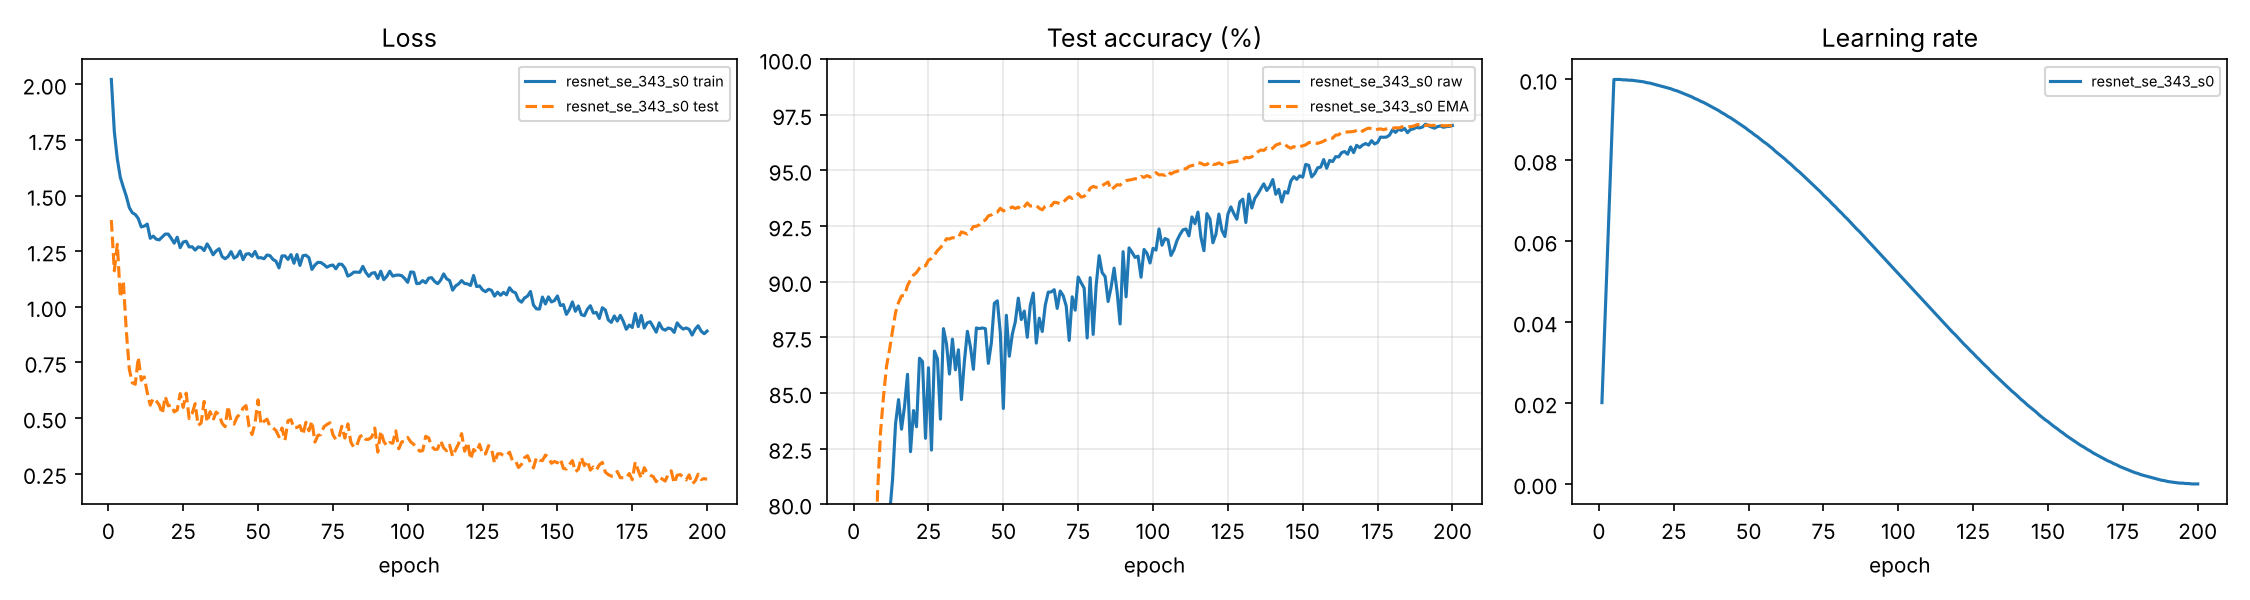
\includegraphics[width=\textwidth]{figures/curves_s0.png}
\caption{Training of the final model (seed 0). Left: cross-entropy on mixed/augmented training batches vs.\ clean test images. Middle: CIFAR-10 test accuracy of the raw weights and of the EMA weights. Right: learning-rate schedule. Accuracy improves until the last epoch; the EMA curve is smooth and dominates the raw weights until they converge together.}
\label{fig:curves}
\end{figure}

\begin{table}[h]
\centering\small
\caption{Final results. CIFAR-10 accuracy is on the standard 10{,}000-image test split (never used for training or selection). Kaggle scores are accuracy on the competition's 2{,}000 held-out images (public/private halves).}
\label{tab:results}
\footnotesize
\begin{tabular}{llrrrrr}
\toprule
Run & Model & Params & CIFAR-10 test & + flip TTA & Kaggle public & Kaggle private \\
\midrule
seed 0 (\textbf{final}) & resnet\_se\_343 & 4,988,274 & \textbf{97.00\%} & \textbf{97.20\%} & \textbf{0.891} (rank 49) & \textbf{0.869} (rank 41) \\
seed 1 & resnet\_se\_343 & 4,988,274 & 96.88\% & 97.08\% & -- & -- \\
\bottomrule
\end{tabular}
\end{table}

\textbf{Accuracy.} The final model reaches 97.00\% on the CIFAR-10 test split (97.20\% with flip-TTA) with 4{,}988{,}274 parameters. A second seed reached 96.88\%/97.08\%, so seed-to-seed variance is about $\pm0.1$ points and the result is robust. Per-epoch numbers are in \texttt{checkpoints/resnet\_se\_343\_s0/} (\texttt{log.csv}) and in the executed notebook; the peak EMA accuracy during training was 97.09\% (epoch 190), and the model stayed above 96.5\% for the last 40 epochs.

\textbf{Competition score.} The same model scored 0.891 on the public half and 0.869 on the private half of the competition test set. The 2.2-point difference between the halves is within the sampling noise of 1{,}000 images (standard error $\approx1\%$) and the whole field moved in the same direction; our rank improved from 49 to 41, consistent with having selected the model without reference to the public leaderboard. The gap between 97.2\% and $\sim$0.88 is the CIFAR-10.1 generalization gap discussed in Section~\ref{sec:shift}, in line with the 3--15 point drops reported in the literature.

\textbf{What we would do with more compute.} The code already implements two steps we could not complete before the deadline with a single free T4: (1) a 400-epoch schedule, and (2) knowledge distillation~\cite{hinton2015} of a single $<$5M student from an ensemble of three independently-seeded teachers (\texttt{--teachers}), plus 10-view TTA. Ensembling and distillation reduce variance, which is precisely what the ``accuracy on the line'' analysis suggests is needed to gain on a CIFAR-10.1-style split, and we would expect a few tenths of a point on CIFAR-10 and a somewhat larger gain on the private leaderboard.

\section{Conclusion}
A carefully budgeted three-stage SE-ResNet with 4.99M parameters, trained from scratch with a strong but standard regularization recipe and EMA, achieves 97.0--97.2\% on CIFAR-10 in two GPU-hours. The competition's test set turned out to be a CIFAR-10.1-style shifted set; recognizing this early led us to optimize genuine accuracy and avoid leaderboard overfitting, which was rewarded on the private split. All code, logs and the executed notebook are in the repository linked on page~1.

\begin{thebibliography}{9}\small
\bibitem{he2016} K. He, X. Zhang, S. Ren, J. Sun. Deep Residual Learning for Image Recognition. \emph{CVPR}, 2016.
\bibitem{hu2018} J. Hu, L. Shen, G. Sun. Squeeze-and-Excitation Networks. \emph{CVPR}, 2018.
\bibitem{muller2021} S. M\"uller, F. Hutter. TrivialAugment: Tuning-free Yet State-of-the-Art Data Augmentation. \emph{ICCV}, 2021.
\bibitem{yun2019} S. Yun et al. CutMix: Regularization Strategy to Train Strong Classifiers with Localizable Features. \emph{ICCV}, 2019.
\bibitem{zhang2018} H. Zhang, M. Cisse, Y. Dauphin, D. Lopez-Paz. mixup: Beyond Empirical Risk Minimization. \emph{ICLR}, 2018.
\bibitem{zhong2020} Z. Zhong et al. Random Erasing Data Augmentation. \emph{AAAI}, 2020.
\bibitem{szegedy2016} C. Szegedy et al. Rethinking the Inception Architecture for Computer Vision. \emph{CVPR}, 2016.
\bibitem{loshchilov2017} I. Loshchilov, F. Hutter. SGDR: Stochastic Gradient Descent with Warm Restarts. \emph{ICLR}, 2017.
\bibitem{polyak1992} B. Polyak, A. Juditsky. Acceleration of Stochastic Approximation by Averaging. \emph{SIAM J. Control Optim.}, 1992.
\bibitem{hinton2015} G. Hinton, O. Vinyals, J. Dean. Distilling the Knowledge in a Neural Network. \emph{NeurIPS Workshop}, 2015.
\bibitem{recht2019} B. Recht, R. Roelofs, L. Schmidt, V. Shankar. Do ImageNet Classifiers Generalize to ImageNet? \emph{ICML}, 2019 (introduces CIFAR-10.1).
\bibitem{miller2021} J. Miller et al. Accuracy on the Line: On the Strong Correlation Between Out-of-Distribution and In-Distribution Generalization. \emph{ICML}, 2021.
\bibitem{kuangliu} kuangliu, \texttt{pytorch-cifar}, \url{https://github.com/kuangliu/pytorch-cifar} (BasicBlock structure adapted; MIT License).
\end{thebibliography}
\end{document}
